\documentclass[a4paper,12pt]{article}
\usepackage[top = 2.5cm, bottom = 2.5cm, left = 2.5cm, right = 2.5cm]{geometry}
\usepackage[T1]{fontenc}
\usepackage[utf8]{inputenc}
\usepackage{multirow} 
\usepackage{booktabs} 
\usepackage{graphicx}
\usepackage[spanish]{babel}
\usepackage{setspace}
\setlength{\parindent}{0in}
\usepackage{float}
\usepackage{fancyhdr}
\usepackage{amsmath}
\usepackage{amssymb}
\usepackage{amsthm}
\usepackage[numbers]{natbib}
\newcommand\Mycite[1]{%
	\citeauthor{#1}~[\citeyear{#1}]}
\usepackage{graphicx}
\usepackage{subcaption}
\usepackage{booktabs}
\usepackage{etoolbox}
\usepackage{minibox}
\usepackage{hyperref}
\usepackage{xcolor}
\usepackage[skins]{tcolorbox}
%---------------------------

\newtcolorbox{cajita}[1][]{
	 #1
}

\newenvironment{sol}
{\renewcommand\qedsymbol{$\square$}\begin{proof}[\textbf{Solución.}]}
	{\end{proof}}

\newenvironment{dem}
{\renewcommand\qedsymbol{$\blacksquare$}\begin{proof}[\textbf{Demostración.}]}
	{\end{proof}}

\newtheorem{problema}{Problema}
\newtheorem{definicion}{Definición}
\newtheorem{ejemplo}{Ejemplo}
\newtheorem{teorema}{Teorema}
\newtheorem{corolario}{Corolario}[teorema]
\newtheorem{lema}[teorema]{Lema}
\newtheorem{prop}{Proposición}
\newtheorem*{nota}{\textbf{NOTA}}
\renewcommand\qedsymbol{$\blacksquare$}
\usepackage{svg}
\usepackage{tikz}
\usepackage[framemethod=default]{mdframed}
\global\mdfdefinestyle{exampledefault}{%
linecolor=lightgray,linewidth=1pt,%
leftmargin=1cm,rightmargin=1cm,
}




\newenvironment{noter}[1]{%
\mdfsetup{%
frametitle={\tikz\node[fill=white,rectangle,inner sep=0pt,outer sep=0pt]{#1};},
frametitleaboveskip=-0.5\ht\strutbox,
frametitlealignment=\raggedright
}%
\begin{mdframed}[style=exampledefault]
}{\end{mdframed}}
\newcommand{\linea}{\noindent\rule{\textwidth}{3pt}}
\newcommand{\linita}{\noindent\rule{\textwidth}{1pt}}

\AtBeginEnvironment{align}{\setcounter{equation}{0}}
\pagestyle{fancy}

\fancyhf{}









%----------------------------------------------------------
\lhead{\footnotesize Data Mining}
\rhead{\footnotesize  Armas, Billingslea, Rompich}
\cfoot{\footnotesize \thepage}


%--------------------------

\begin{document}
 \thispagestyle{empty} 
    \begin{tabular}{p{15.5cm}}
    \begin{tabbing}
    \textbf{Universidad del Valle de Guatemala} \\
    Ejercicio en clase - Grupo 5 \\\\

   \textbf{Estudiante:} Esteban Armas, Jackelin Billingslea, Rudik Rompich\\
   \textbf{Correos:} \href{mailto:arm19371@uvg.edu.gt}{arm19371@uvg.edu.gt},\href{mailto:bil19161@uvg.edu.gt}{bil19161@uvg.edu.gt}, \href{mailto:rom19857@uvg.edu.gt}{rom19857@uvg.edu.gt}\\
   \textbf{Carnés:} 19371, 19161, 19857
    \end{tabbing}
    \begin{center}
        IA3028 - Data Mining - Catedrático: Luis Pedro Flores\\
        \today
    \end{center}\\
    \hline
    \\
    \end{tabular} 
    \vspace*{0.3cm} 
    \begin{center} 
    {\Large \bf  PowerBI + Estadística Descriptiva
} 
        \vspace{2mm}
    \end{center}
    \vspace{0.4cm}
%--------------------------

Preguntas a responder: 

\begin{enumerate}
	\item¿Qué influía más en que un pasajero sobreviviera?
	\begin{sol}
		Los siguientes factores fueron determinantes:
		\begin{enumerate}
			\item Pclass (la clase que el pasajero ocupaba). 
		Según la Figura 1, la clase fue uno de los factores más elementales para determinar la supervivencia. Si se pertenecía a la primera clase las probabilidades eran muy altas, en la segunda eran indistintas y en la tercera era casi una condena de muerte. 
		
			\item Sex (el sexo del pasajero).  El sexo fue uno de los factores que determinar la supervivencia. Cabe resaltar que la mayoría de los pasajeros a bordo eran hombres; los cuales murieron en su mayoría. 
			
			\item Fare (la tarifa del pasaje). La tarifa es algo interesante para resaltar, ya que la mayoría de pasajes vendidos fueron los más baratos y 
			en donde más se produjeron muertes. Por lo tanto, un pasaje más caro implicaba una muerte casi segura. 
			\item Embarked (lugar de embarque al Titanic). Aunque intuitivamente el lugar de abordaje no debería implicar nada; cabe resaltar que las muertes que más se produjeron fueron de las personas que embarcaron en Southampton (la ciudad de origen). 
		\end{enumerate}
	Factores que no tuvieron ninguna implicación: 
	\begin{enumerate}
		\item  Age (edad). Pareciera indicar que el factor de la edad no fue determinante para sobrevivir o no.  
	\end{enumerate}
	\end{sol}
	\item ¿Qué \% de pasajeros sobrevivieron?
	\begin{sol}
		Según la Figura 1 el 38.38\% de los pasajeros sobrevivieron. 
\begin{figure}[ht]
	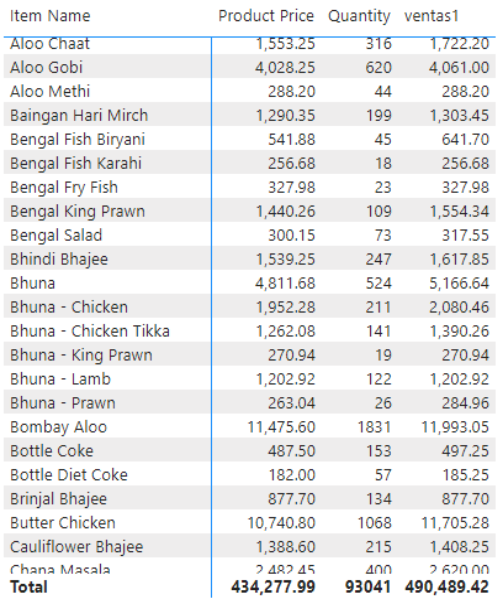
\includegraphics[scale=0.4]{images/1}
	\centering 
	\caption{0 es muerto; 1 es sobreviviente.}
\end{figure}
	\end{sol}
	\item Haga un modelo que pueda predecir la probabilidad de que los pasajeros sobrevivan.
	\begin{sol} 
		Se evaluaron 3 modelos: kNN, Logistic Refression y Tree.
		\begin{figure}[ht]
			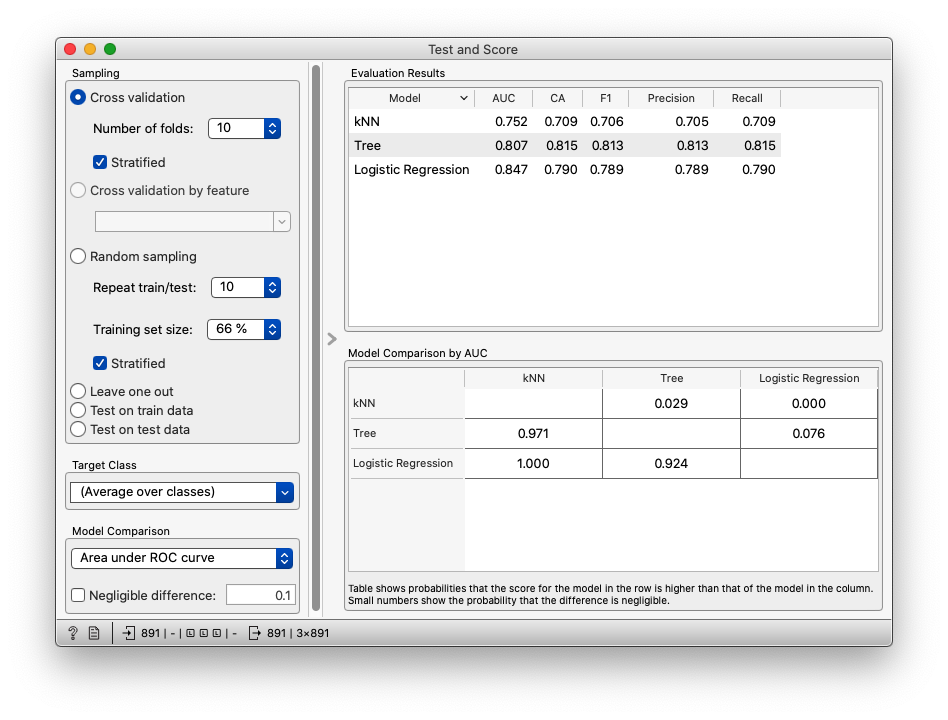
\includegraphics[scale=0.35]{images/8}
			\centering 
			\caption{Modelo kNN, Logistic Regression, Tree.}
		\end{figure}
	\end{sol}
	\item Hay datos de pasajeros que no se tiene el “tag” si sobrevivieron o no. Corra el modelo para entender si los pasajeros sobrevivieron.
	\begin{sol}
		A continuación se observa un pequeño resumen de los datos de acuerdo a la predicción del modelo: 
		\begin{figure}[ht]
			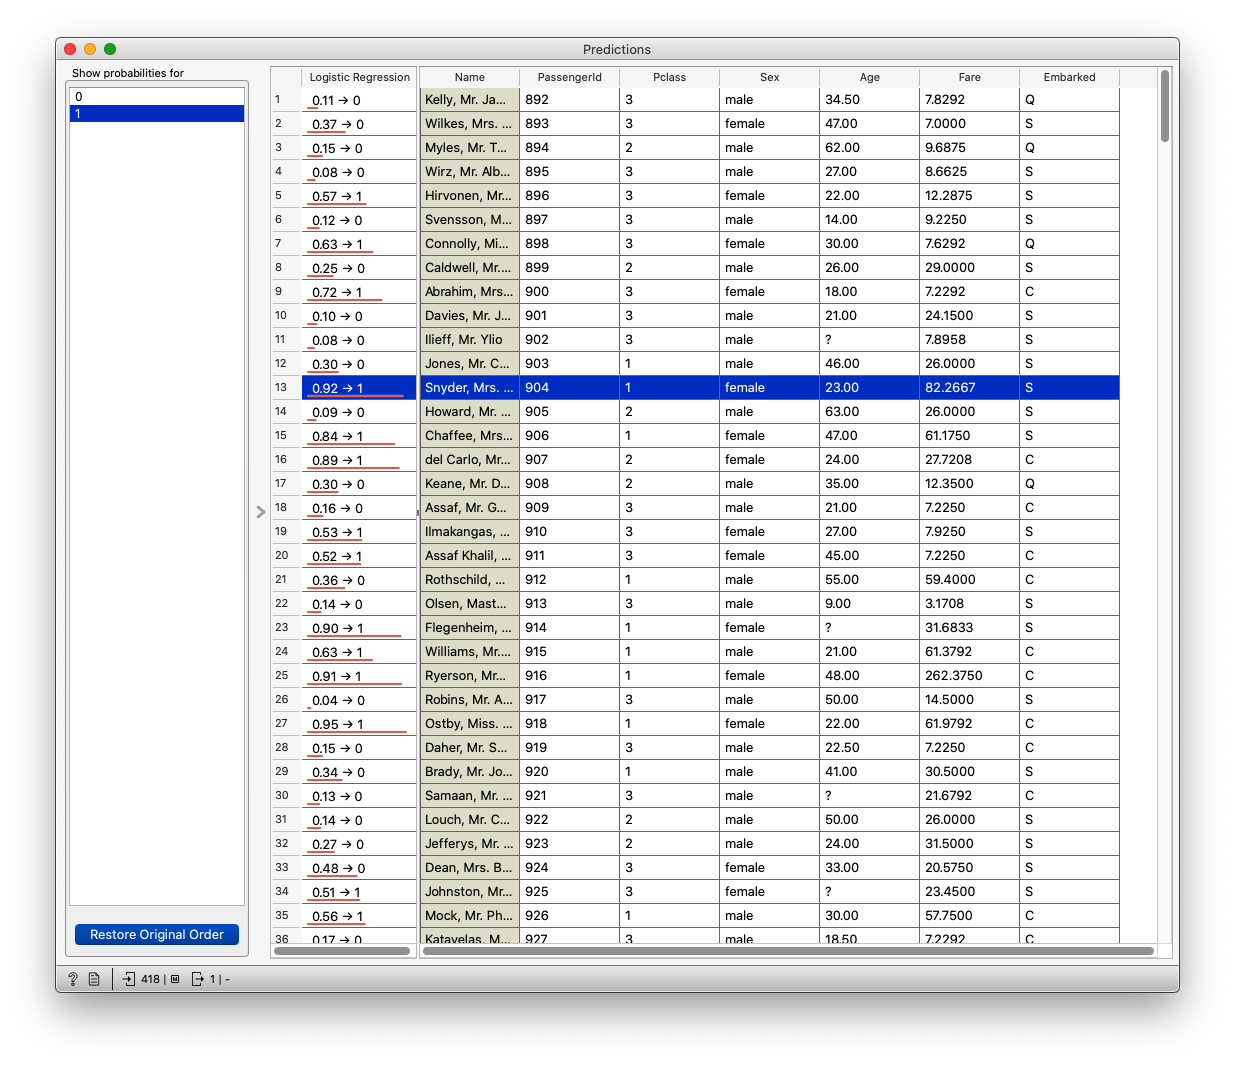
\includegraphics[scale=0.4]{images/9}
			\centering 
			\caption{Predicción}
		\end{figure}
	\end{sol}
\end{enumerate}

	\begin{figure}[ht]
	\begin{subfigure}{.5\textwidth}
		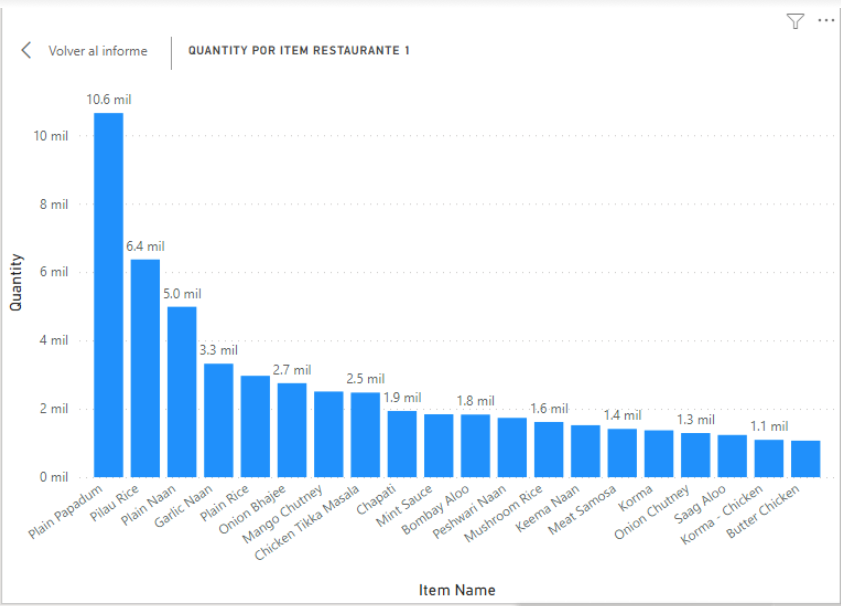
\includegraphics[scale=0.3]{images/2}
		\centering 
		\caption{Frecuencia de sobrevivientes.}
	\end{subfigure}
	\begin{subfigure}{.5\textwidth}
		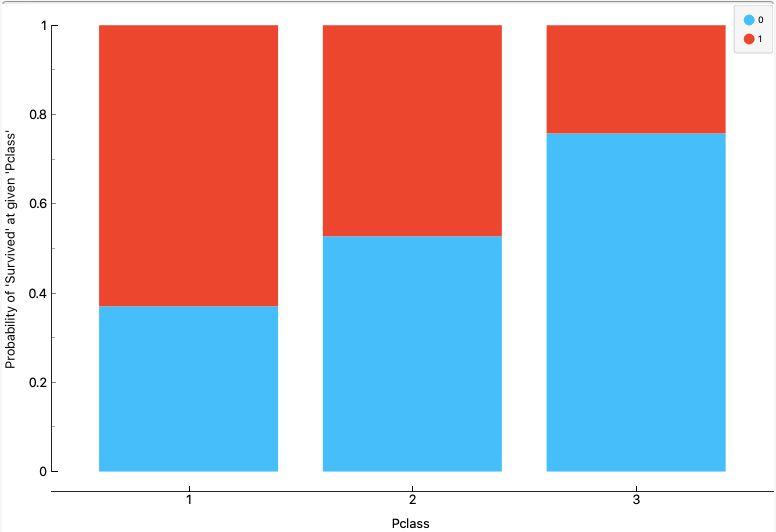
\includegraphics[scale=0.3]{images/3}
		\centering 
		\caption{Probabilidad de sobrevivir.}
	\end{subfigure}
	\caption{Clase}
\end{figure}


\begin{figure}[ht]
	\begin{subfigure}{.5\textwidth}
		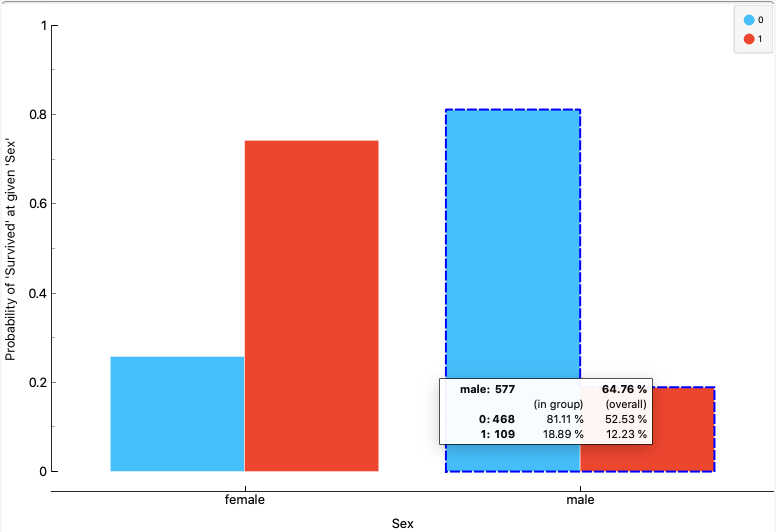
\includegraphics[scale=0.3]{images/4}
		\centering 
		\caption{Probabilidad de sobrevivir.}
	\end{subfigure}
	\begin{subfigure}{.5\textwidth}
		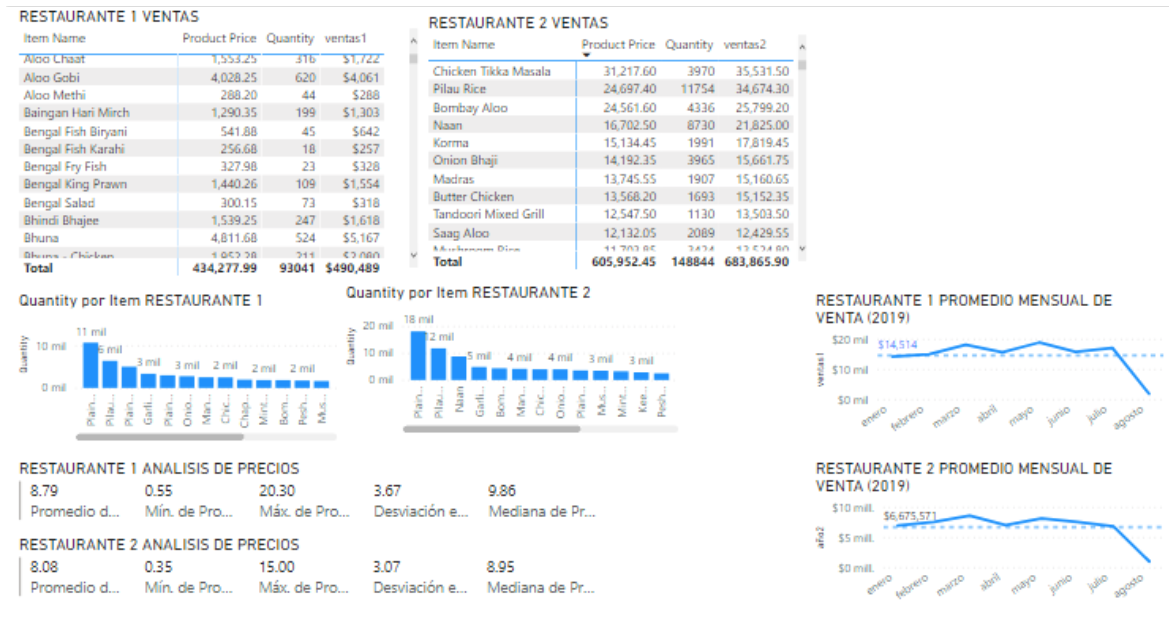
\includegraphics[scale=0.3]{images/5}
		\centering 
		\caption{Sobrevivientes.}
	\end{subfigure}
	\caption{Sexo}
\end{figure}

\begin{figure}[ht]
	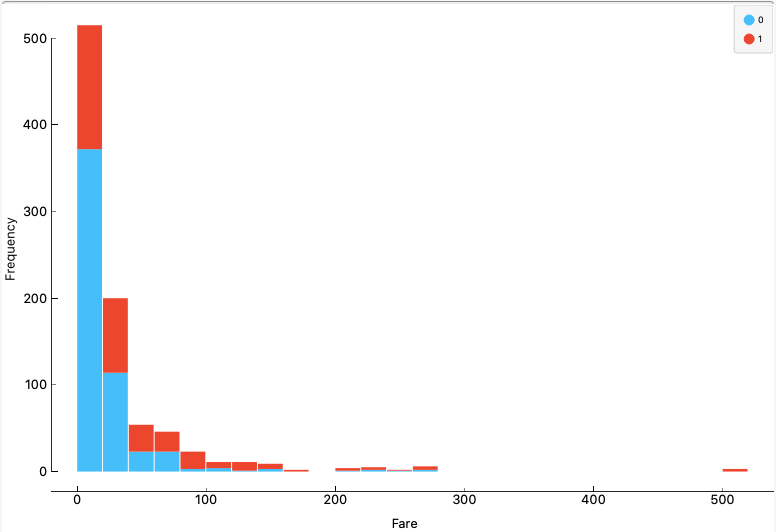
\includegraphics[scale=0.4]{images/6}
	\centering 
	\caption{Fare (tarifa).}
\end{figure}
\begin{figure}[ht]
	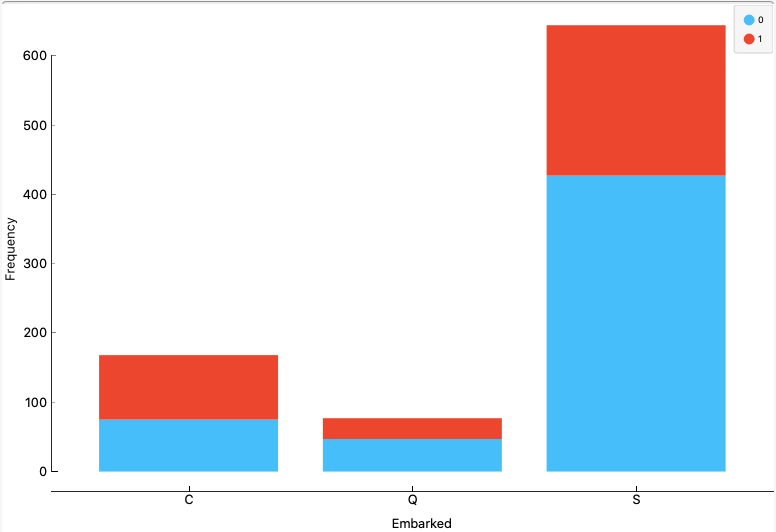
\includegraphics[scale=0.4]{images/7}
	\centering 
	\caption{Embarked (embarque).}
\end{figure}
%---------------------------
%\bibliographystyle{apa}
%\bibliography{referencias.bib}

\end{document}